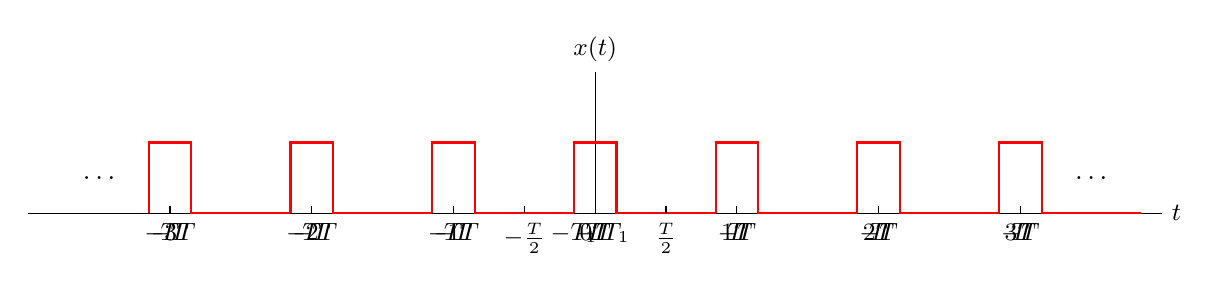
\begin{tikzpicture}[scale=0.9]
	\def\xmin{-7}
	\def\xmax{7}
	\def\ymin{0}
	\def\ymax{2}
	\def\period{2.0}
	\def\T1{0.3}
	\def\A{1}
	
	\edef\pulse{|- ++(2*\T1, \A) |- ++( \period - 2*\T1, -\A)}

	
	\draw (\xmin-1, 0) --(\xmax+1, 0) node[anchor=west] {\small $t$};
	\draw (0, \ymin) --(0, \ymax) node[anchor=south] {\small $x(t)$};
		\foreach \x in {-3, -2, ..., 3}
		{
			\pgfmathmultiply{\period}{\x}
			\edef\position{\pgfmathresult}
			\ifthenelse{\x=0 \OR \x=1 \OR \x=-1}
			{
				%\node at (\position, 0) [anchor=north] {\small $0$};
			}
			{
				
				\node at (\position, 0) [anchor=north] {\small $\x T$};
			}
			\ifthenelse{ \x=1 }
			{
				\node at (\position, 0) [anchor=north] {\small $T$};
			}
			{
			}
			
			\ifthenelse{ \x=-1 }
			{
				\node at (\position, 0) [anchor=north] {\small $-T$};
			}
			{
			}			
			\draw[thick, red] (\position-\T1, 0) \pulse;	
			\draw (\position, 0) -- ++(0,0.1);
			%\pulse{3}{0.4};		
		}
		
		\node at (-\T1, 0) [anchor=north] {\small $-T_1$};
		\node at (\T1, 0) [anchor=north] {\small $T_1$};
		\node at (-\period/2, 0) [anchor=north] {\small $-\frac{T}{2}$};
		\node at (\period/2, 0) [anchor=north] {\small $\frac{T}{2}$};
		\draw (-\period/2, 0) -- ++(0,0.1);
		\draw (\period/2, 0) -- ++(0,0.1);

		\node at (\xmin, \A/2) {$\dots$};
		\node at (\xmax, \A/2) {$\dots$};
\end{tikzpicture}
